\documentclass[tikz,border=4pt]{standalone}
% Shared TikZ style for lecture figures
\usepackage{amsmath,amssymb}
\usepackage{tikz}
\usetikzlibrary{arrows.meta,calc,decorations.pathreplacing,patterns}
\definecolor{teal}{RGB}{38,150,140}
\definecolor{coral}{RGB}{230,95,75}
\definecolor{ink}{RGB}{20,45,60}
\tikzset{
  >={Stealth[length=2.6mm]},
  every picture/.style={line cap=round,line join=round,thick,ink},
  map/.style={->,thick},
  dot/.style={circle,fill,inner sep=1.2pt},
}

\begin{document}
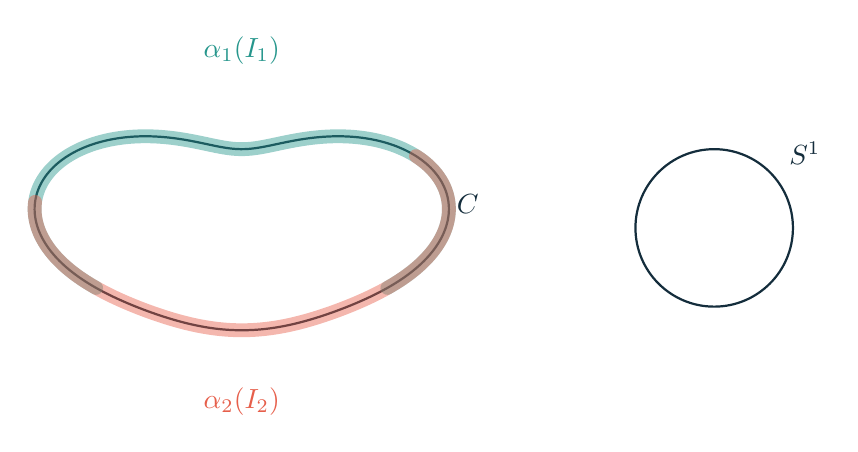
\begin{tikzpicture}[declare function={rho(\t)=1.5+0.35*cos(2*\t)+0.15*sin(3*\t);}]
  % the closed curve
  \draw[thick] plot[domain=0:360,samples=180,smooth cycle,variable=\t]
    ({1.4*rho(\t)*cos(\t)},{rho(\t)*sin(\t)});
  % two overlapping parametrized arcs
  \draw[teal,line width=5pt,opacity=0.45] plot[domain=-30:210,samples=120,smooth,variable=\t]
    ({1.4*rho(\t)*cos(\t)},{rho(\t)*sin(\t)});
  \draw[coral,line width=5pt,opacity=0.45] plot[domain=170:390,samples=120,smooth,variable=\t]
    ({1.4*rho(\t)*cos(\t)},{rho(\t)*sin(\t)});
  \node[teal] at (0,2.25) {$\alpha_{1}(I_{1})$};
  \node[coral] at (0,-2.2) {$\alpha_{2}(I_{2})$};
  \node at (2.6,0.3) [right] {$C$};
  % the abstract model S^1
  \begin{scope}[xshift=6cm]
    \draw[thick] (0,0) circle (1);
    \node at (1.15,0.95) {$S^{1}$};
  \end{scope}
\end{tikzpicture}
\end{document}
